\chapter{Конструкторская часть}

В данном разделе будут представлены схемы реализаций алгоритмов умножения матриц, среди которых стандартный, Винограда и Винограда с улучшениями.

\section{Разработка стандартного алгоритма умножения матриц}
На рисунке \ref{img:stand} представлена схема реализации стандартного алгоритма умножения матриц.

\begin{figure}[h!]
    \centering
    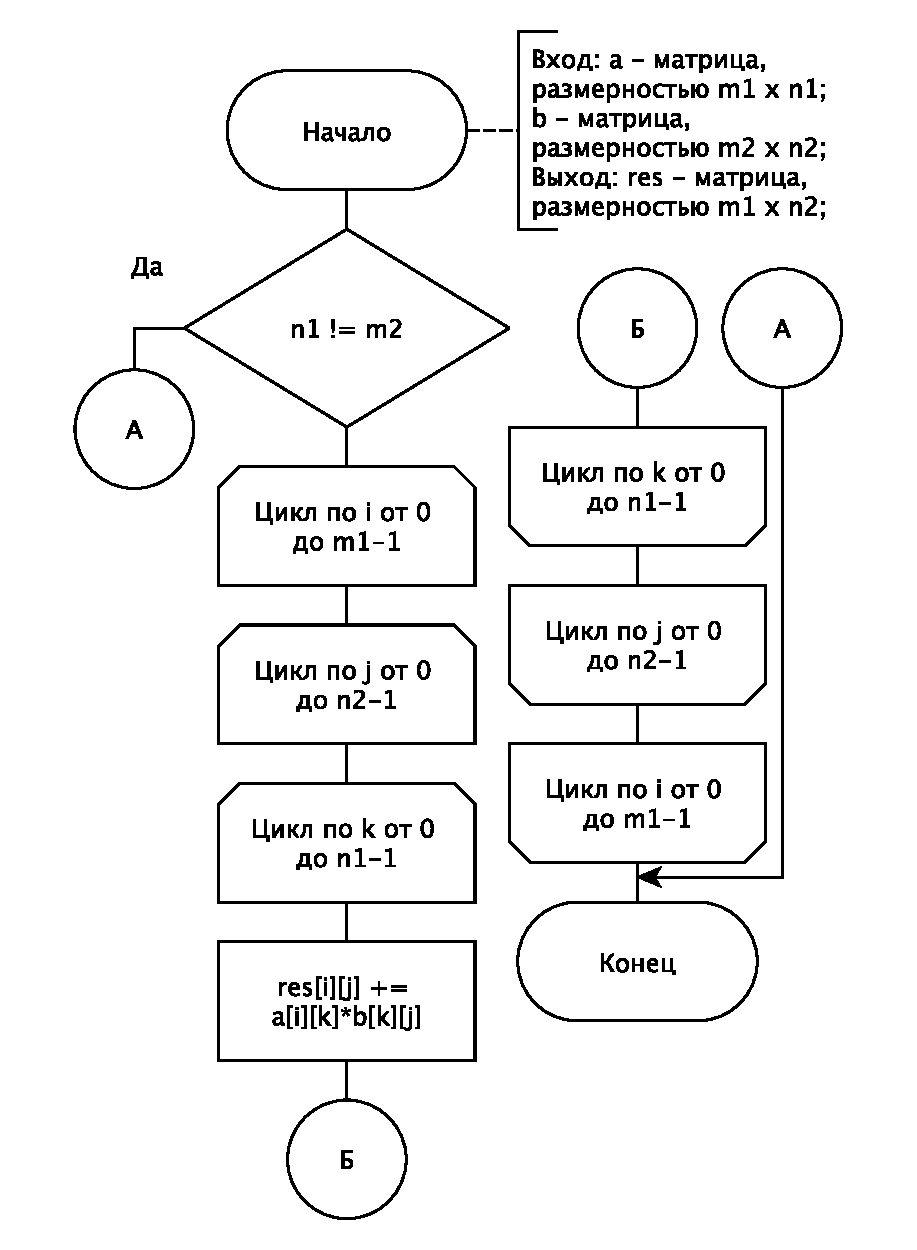
\includegraphics[width=0.6\linewidth]{stand.pdf}
    \caption{Схема реализации стандартного алгоритма умножения матриц}
    \label{img:stand}
\end{figure}

\section{Разработка алгоритма Винограда умножения матриц}
На рисунке \ref{img:win} представлена схема реализации алгоритма Винограда умножения матриц. На рисунках \ref{img:rc} и \ref{img:cc} представлены схемы реализаций алгоритмов подпрограмм поиска произведений соседних элементов строк матрицы (рисунок \ref{img:rc}) и поиска произведений соседних элементов столбцов матрицы (рисунок \ref{img:cc}), необходимых для реализации алгоритма Винограда умножения матриц.

\begin{figure}[h!]
    \centering
    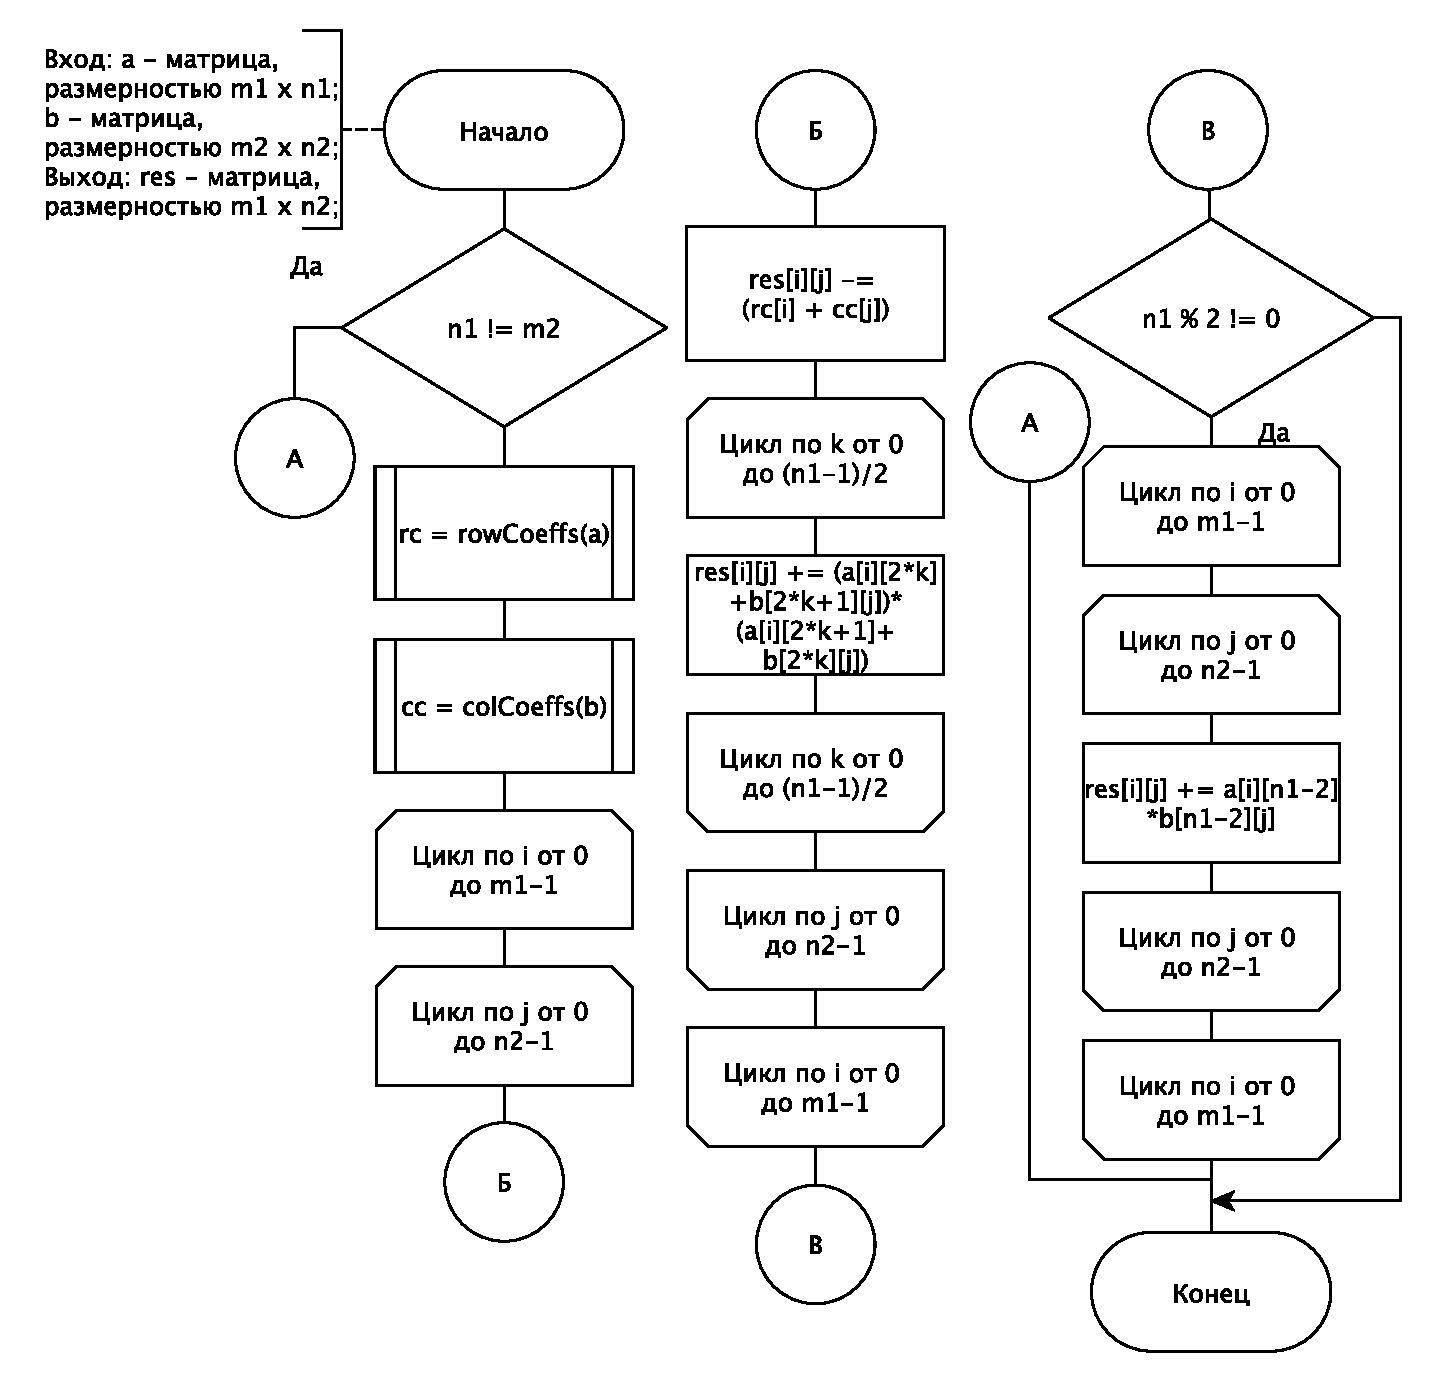
\includegraphics[width=1\linewidth]{win.pdf}
    \caption{Схема реализации алгоритма Винограда умножения матриц}
    \label{img:win}
\end{figure}

\begin{figure}[h!]
    \centering
    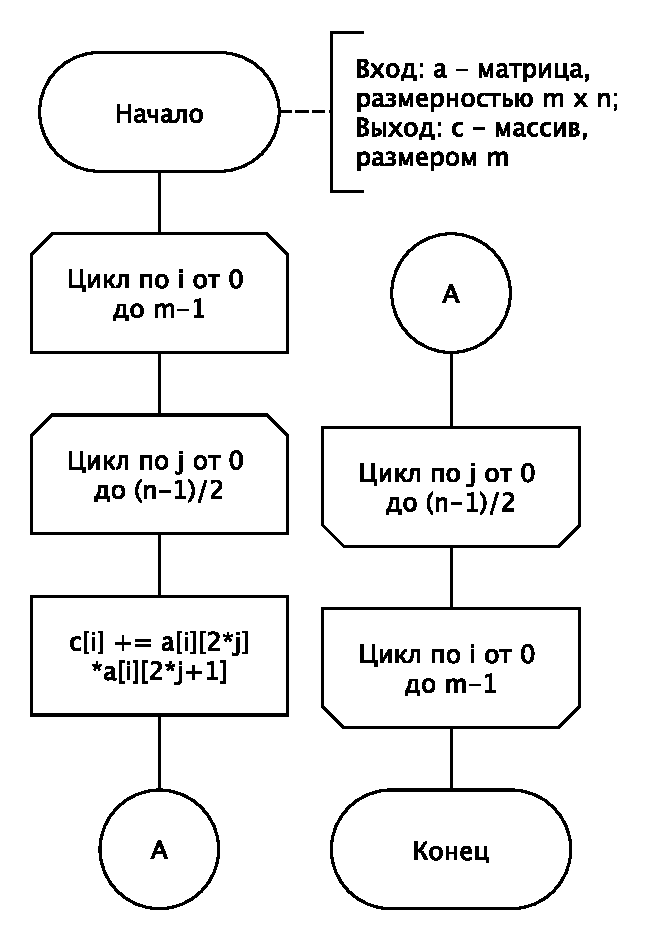
\includegraphics[width=0.38\linewidth]{rc.pdf}
    \caption{Схема реализации алгоритма поиска произведений соседних элементов строк матрицы}
    \label{img:rc}
\end{figure}

\begin{figure}[h!]
    \centering
    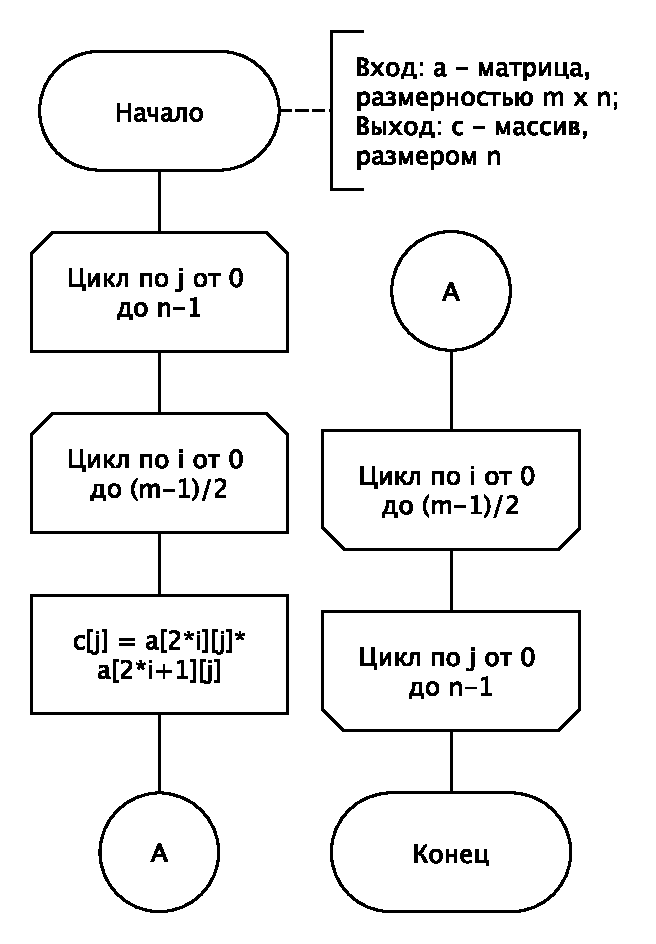
\includegraphics[width=0.38\linewidth]{cc.pdf}
    \caption{Схема реализации алгоритма поиска произведений соседних элементов столбцов матрицы}
    \label{img:cc}
\end{figure}

\newpage

\section{Разработка оптимизированного алгоритма Винограда умножения матриц}
На рисунке \ref{img:winBetter} представлена схема реализации оптимизированного алгоритма Винограда умножения матриц. На рисунке \ref{img:rcccBetter} представлены схемы реализаций алгоритмов подпрограмм улучшенного поиска произведений соседних элементов строк матрицы и улучшенного поиска произведений соседних элементов столбцов матрицы, необходимых для реализации оптимизированного алгоритма Винограда умножения матриц.

\begin{figure}[h!]
    \centering
    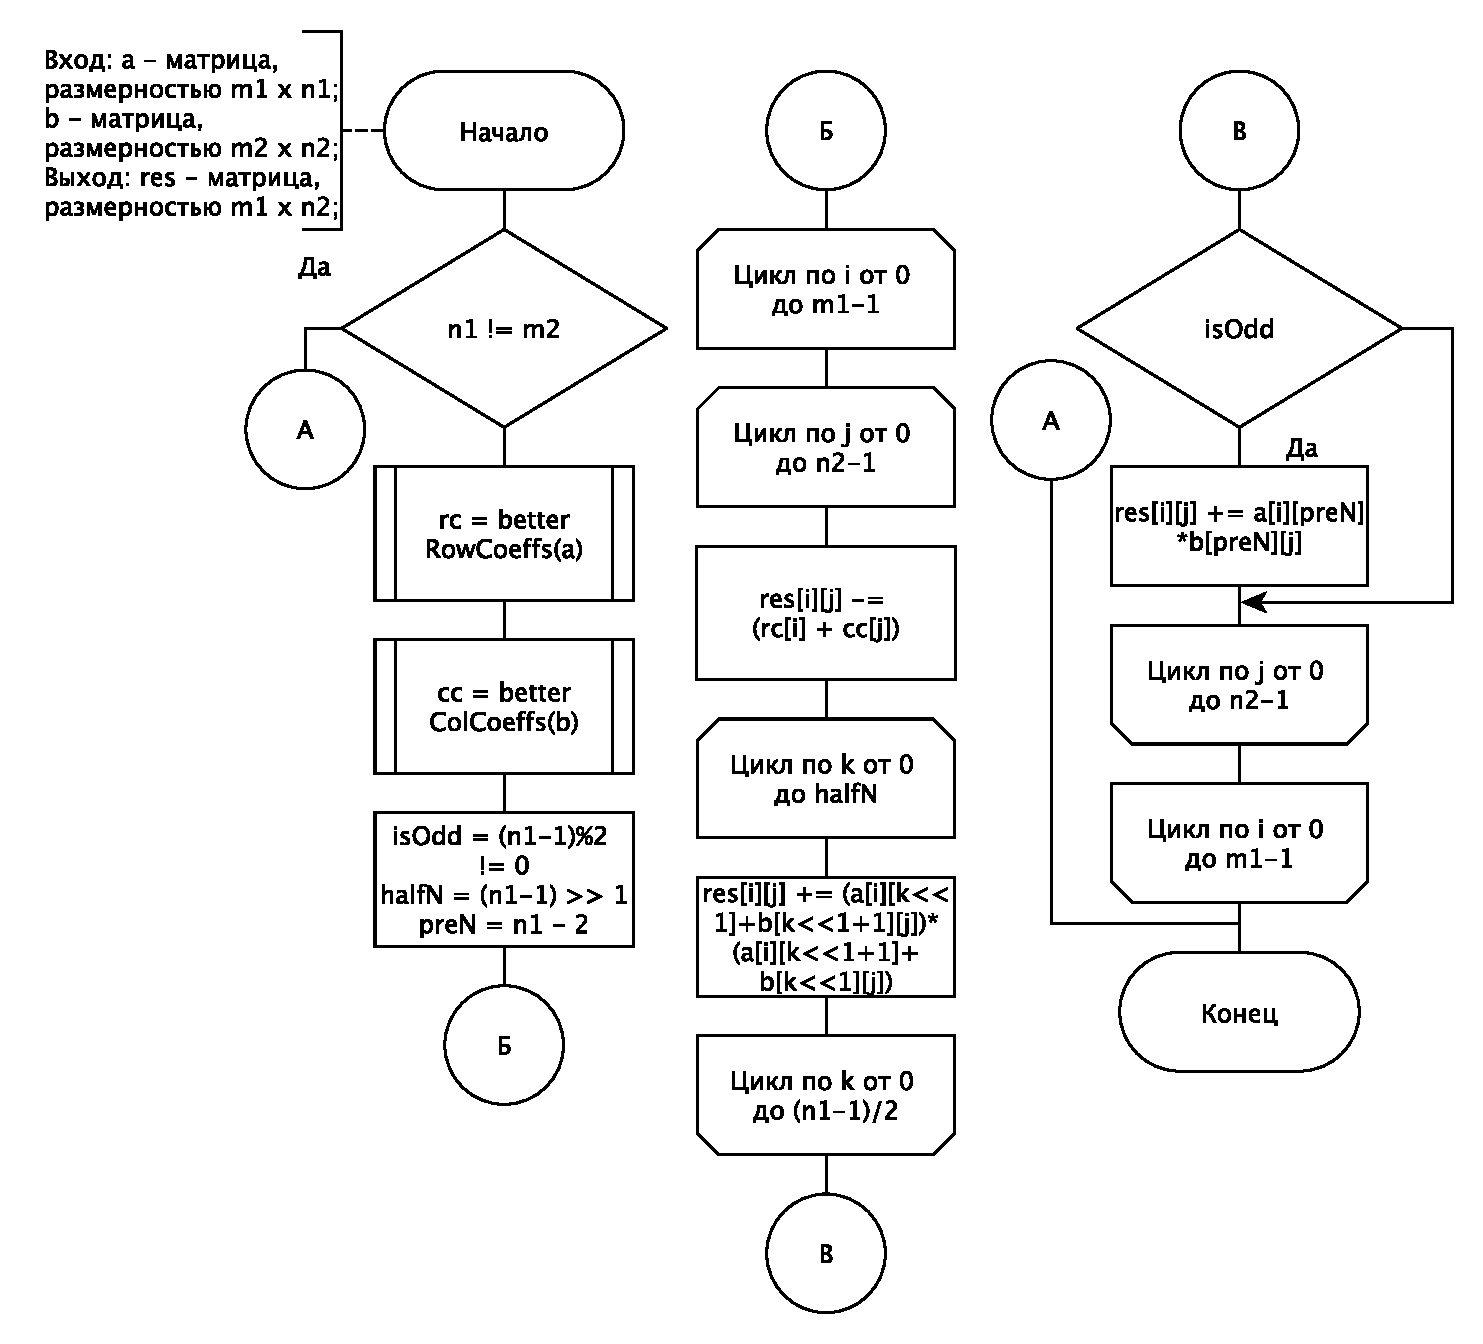
\includegraphics[width=1\linewidth]{winBetter.pdf}
    \caption{Схема реализации оптимизированного алгоритма Винограда умножения матриц}
    \label{img:winBetter}
\end{figure}

\begin{figure}[h!]
    \centering
    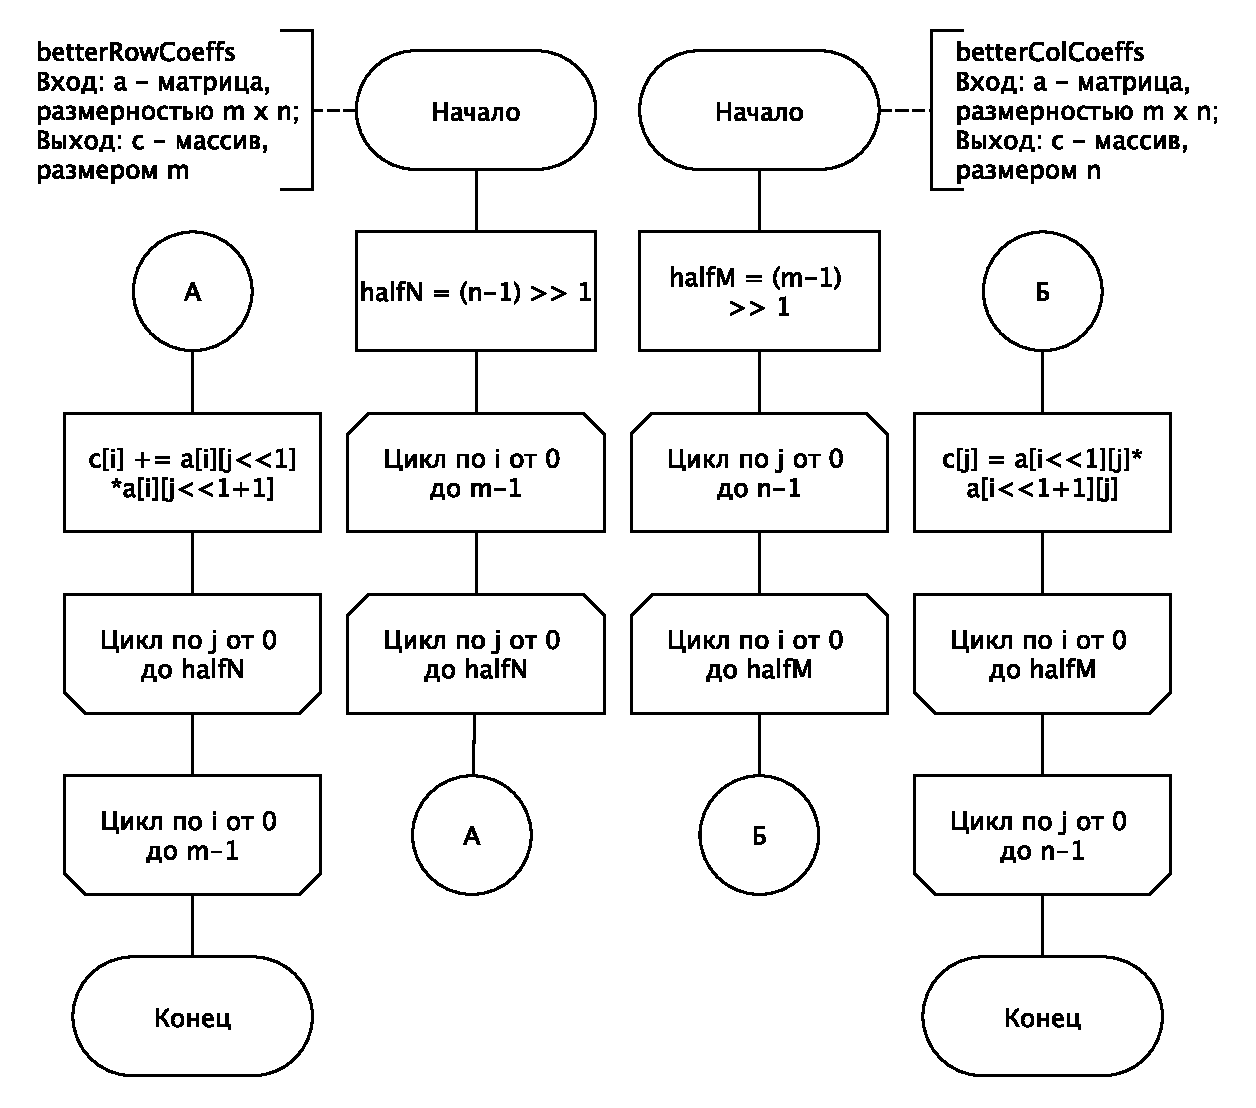
\includegraphics[width=0.9\linewidth]{rcccBetter.pdf}
    \caption{Схема реализации улучшенного поиска произведений соседних элементов строк и столбцов матрицы}
    \label{img:rcccBetter}
\end{figure}

\newpage

\section{Модель вычислений}
Для вычисления трудоёмкости данных алгоритмов необходимо ввести модель вычислений.

Обозначим трудоёмкость как $f_{a}$, где $a$~---~индекс, указывающий операцию, блок кода или оператор, для которого вычисляется трудоёмкость.

Определим трудоёмкость базовых операций как:
\begin{equation}
\begin{array}{rrrr}
	f_{+}=1 & \quad f_{-}=1 & \quad f_{+=}=1 & \quad f_{-=}=1 \\
	f_{:=}=1 & \quad f_{<<}=1 & \quad f_{>>}=1 & \quad f_{[]}=1 \\
	f_{++}=1 & \quad f_{--}=1 & \quad f_{>}=1 & \quad f_{<}=1 \\
	f_{>=}=1 & \quad f_{<=}=1 & \quad f_{!=}=1 & \quad f_{==}=1 \\
	f_{\cdot}=2 & \quad f_{/}=2 & \quad f_{\%}=2 & \quad \\
\end{array}
\end{equation}

Определим трудоёмкость вызова функции как $0$.

Определим трудоёмкость условия как

\begin{equation}
	f_{if} = f_{cc} + \begin{cases}
		\min(f_1, f_2),& \text{в лучшем случае}, \\
		\max(f_1, f_2),& \text{в худшем случае},
	\end{cases}
\end{equation}
где приняты следующие обозначения:
\begin{itemize}
	\item $f_{cc}$~---~трудоёмкость вычисления условия;
	\item $f_1$~---~трудоёмкость блока после $if$;
	\item $f_2$~---~трудоёмкость блока после $else$.
\end{itemize}

Определим трудоёмкость цикла как
\begin{equation}
	f_{loop} = f_{init} + f_{first-cmp} + n \cdot (f_{body} + f_{inc} + f_{cmp}),
\end{equation}
где приняты следующие обозначения:
\begin{itemize}
	\item $f_{init}$~---~трудоёмкость инициализации;
	\item $f_{first-cmp}$~---~трудоёмкость первого сравнения;
	\item $f_{body}$~---~трудоёмкость тела цикла;
	\item $n$~---~количество итераций цикла;
	\item $f_{inc}$~---~трудоёмкость изменения индекса;
	\item $f_{cmp}$~---~трудоёмкость сравнения.
\end{itemize}

\section{Трудоёмкость алгоритмов умножения матриц}
Введём некоторые обозначения:
\begin{itemize}
	\item $M$~---~размерность первой матрицы по количеству строк;
	\item $N$~---~размерность второй матрицы по количеству столбцов;
	\item $K$~---~размерность первой матрицы по количеству столбцов (второй матрицы по количеству строк);
	\item $f_{best}$~---~трудоёмкость алгоритма в лучшем случае;
	\item $f_{worst}$~---~трудоёмкость алгоритма в худшем случае.
\end{itemize}

\subsection{Трудоёмкость стандартного алгоритма умножения матриц}
Далее приведён расчёт трудоёмкость алгоритма алгоритма умножения матриц. Для данного алгоритма не выделяются худший и лучший случаи в связи с тем, что его быстродействие зависит лишь от размерности исходных матриц.

Трудоёмкость стандартного алгоритма умножения матриц включает в себя:
\begin{itemize}
	\item трудоёмкость внешнего цикла по $i = \overline{0,M-1}$: \begin{equation} \label{eqn:i-loop}
		f_{i-loop} = 2 + M \cdot (2 + f_{body});
	\end{equation}
	\item трудоёмкость внутреннего цикла по $j = \overline{0..N-1}$: \begin{equation}
		f_{j-loop} = 2 + N \cdot (2 + f_{body});
	\end{equation}
	\item трудоёмкость внутреннего цикла по $k = \overline{0..K-1}$: \begin{equation}
		f_{k-loop} = 2 + K \cdot (2 + 12).
	\end{equation}
\end{itemize}

Так как трудоёмкость стандартного алгоритма умножения матриц равна трудоёмкости внешнего цикла, можно вычислить ее, подставив в (\ref{eqn:i-loop}) трудоёмкости внутренних циклов:
\begin{equation}
	\label{for:standard}
	f_{standard} = 2 + M \cdot (4 + N \cdot (4 + 14 \cdot K)).
\end{equation}

%куда подставить
% еще там где-то две формулы с двоеточием

Таким образом, для стандартного алгоритма умножения матриц трудоёмкость составит:
\begin{equation}
	f_{standard} = 2 + 4 \cdot M + 4 \cdot M \cdot N + 14 \cdot M \cdot N \cdot K \approx 14 \cdot M \cdot N \cdot K.
\end{equation}

Такую трудоёмкость можно оценить как $O(M \cdot N \cdot K)$.

\subsection{Трудоёмкость алгоритма Винограда для умножения матриц} \label{tv}
Далее приведён расчёт трудоёмкости алгоритма Винограда для умножения матриц. Лучшим случаем считается ситуация, когда размерность исходной матрицы чётная, и худшим, когда нечётная.
% M + 2 + 4M + 17M(K/2) + N + 2 + 4N + 17N(K/2) + 2 + 4M + 13MN + 30MN(K/2) + 
% 3 OR 2 + 4M + 16MN

Трудоёмкость алгоритма Винограда включает в себя:
\begin{itemize}
	\item трудоёмкость создания и заполнения массивов $rowCoeffs$ и $colCoeffs$:
	\begin{equation}
		f_{rowCoeffs} = M + (2 + M \cdot (5 + \frac{K}{2} \cdot 18)),
	\end{equation}
	\begin{equation}
		f_{colCoeffs} = N + (2 + N \cdot (5 + \frac{K}{2} \cdot 18));
	\end{equation}
	\item трудоёмкость цикла заполнения матрицы-результата для чётных размеров исходной матрицы:
	\begin{equation}
		f_{loop} = 2 + M \cdot (4 + N \cdot (14 + \frac{K}{2} \cdot 31));
	\end{equation}
	\item трудоёмкость цикла для дополнения умножения суммой последних нечётных строки и столбца при нечётном размере исходной матрицы:
	\begin{equation}
		f_{loop-odd} = 3 + \begin{cases}
			0, & \text{если размер чётный,}\\
			2 + M \cdot (4 + N \cdot 16), & \text{иначе.}
		\end{cases}
	\end{equation}
\end{itemize}
	
Таким образом, для худшего случая (нечётный общий размер матриц) трудоёмкость составит:
\begin{equation}
	\label{for:bad}
	f_{Win-worst} \approx 15.5 \cdot M \cdot N \cdot K = O(M \cdot N \cdot K),
\end{equation}

а лучшего случая (чётный общий размер матриц) трудоёмкость составит:
\begin{equation}
	\label{for:good}
	f_{Win-best} \approx 15.5 \cdot M \cdot N \cdot K = O(M \cdot N \cdot K).
\end{equation}

\subsection{Трудоёмкость оптимизированного алгоритма Винограда для умножения матриц}
Рассчитаем трудоёмкость оптимизированного алгоритма Винограда для умножения матриц. Как и для обычного алгоритма Винограда (см. п. \ref{tv}), лучшим случаем считается ситуация, когда размерность исходной матрицы чётная, и худшим, когда нечётная. Применённые улучшения приведены в пункте \ref{better}

Трудоёмкость оптимизированного алгоритма Винограда включает в себя:
\begin{itemize}
	\item трудоёмкость создания и заполнения массивов $rowCoeffs$ и $colCoeffs$:
	\begin{equation}
		f_{rowOCoeffs} = M + 2 + (2 + M \cdot (4 + \frac{K}{2} \cdot 15)),
	\end{equation}
	\begin{equation}
		f_{colOCoeffs} = N + (2 + N \cdot (4 + \frac{K}{2} \cdot 15));
	\end{equation}
	\item трудоёмкость предвычисления переменных: $f_{val} = 5$;
	\item трудоёмкость цикла заполнения матрицы-результата для чётных размеров исходной матрицы с учётом ситуации с нечётным размером:
	\begin{equation}
		f_{loopO} = 2 + M \cdot (4 + N \cdot (17 + \frac{K}{2} \cdot 23)).
	\end{equation}
\end{itemize}
	
Таким образом, для худшего случая (нечётный общий размер матриц) трудоёмкость составит:
\begin{equation}
	\label{for:bad}
	f_{WinO-worst} \approx 11.5 \cdot M \cdot N \cdot K = O(M \cdot N \cdot K),
\end{equation}

а лучшего случая (чётный общий размер матриц) трудоёмкость составит:
\begin{equation}
	\label{for:good}
	f_{WinO-best} \approx 11.5 \cdot M \cdot N \cdot K = O(M \cdot N \cdot K).
\end{equation}

\newpage